\documentclass{article}[12pt]
\renewcommand{\baselinestretch}{1.5}
\setlength{\parskip}{1em}

\usepackage[parfill]{parskip}
\usepackage[affil-it]{authblk}
\usepackage[space]{grffile}

\usepackage[a4paper]{geometry}
\geometry{verbose}
\usepackage{float}
\usepackage{graphicx}
\graphicspath{{figures/}}
\usepackage{setspace}
\usepackage{caption}

\usepackage[utf8]{inputenc}
\usepackage[english]{babel}

\usepackage{latexsym,textcomp,longtable,tabulary}
\usepackage{booktabs,array,multirow,braket}
\usepackage{amsfonts,amsmath,amssymb,mathbbol,calc}
\usepackage{subfigure,color,blindtext,enumitem,siunitx}
\usepackage[colorinlistoftodos]{todonotes}

\usepackage{mathtools}
\usepackage{url,hyperref,etoolbox}
\numberwithin{equation}{section}
\hypersetup{colorlinks=false,pdfborder={0 0 0}}

%+figure layout options
\restylefloat{figure}
\setlist{leftmargin=*,before=\setlength{\rightmargin}{\leftmargin}}
%-figure layout options

\providecommand\citet{\cite}
\providecommand\citep{\cite}
\providecommand\citealt{\cite}

\makeatletter
\makeatother

\def\code#1{\texttt{#1}}
\begin{document}

\title{
Time-series segmentation and latent\\ representation of musical instruments
}

\author{Gregory Szep}
\affil{King's College London}
\date{\today}
\maketitle

\abstract{Music information retrieval tasks serve as faithful benchmarks for
time-series analysis pipelines due to the availability of strongly labelled
training data such as MusicNet. Clustering algorithms in spectral sub-spaces,
hidden Markov models and causal convolutional neural networks are compared in
their ability to transform time-series to a continuous latent space that
clusters eleven orchestral instruments. The latent space is evaluated
quantitatively with precision-recall metrics obtained by comparing the
instrument prediction from a segment of audio to the ground truth obtained
from musical scores, and qualitatively by generating samples of audio for given
regions in the latent space.}
\section{scientific publication}
Select a scientific publication about non-equilibrium molecular dynamics of
biomolecules and discuss its relevance respect to the course you attended and
this research assignment.

\section{Analysis of Umbrella Sampling simulations}
Every student has access to the raw data of umbrella sampling simulations for
two systems. These umbrella sampling simulations have been ran having the
aim to calculate the Potential of Mean Force (PMF) of the mechanical unfolding
of two peptides: one being in the initial conformational state of an a-helix; the
other being in the initial conformational state of a b-hairpin. Every student is
supposed to calculate the PMF for both the systems
\subsection{Describe the simulated systems and the type of performed simulations you
analyze}
\subsection{Calculate and display (plot) the PMF for the two systems. Explore the
relevance of the bootstrap parameter respect to evaluation of the PMF’s error
using the script g_wham_script_new.x}

Bootstrapping is a resampling method that quantifies statistical uncertainty by
dividing the data into $N$ subsets, hence without additional measruements
uncertainty is obtained by \textit{pulling the data up by its own bootstraps}.
By default the \code{g\_wham} code forms subsets with replacement over the
complete histograms along the reaction coordinate \cite{gwham2010}, leaving us
with $N$ as a hyperparameter.
\\\\
This hyperparameter is subject to the bias-variance trade-off. Chooseing a large
$N$ results in relatively unbiased and uncertain estimates, while a small number
of subsets give rise to more certain yet biased estimates. The former is
preferred but comes with a computational cost. It appears that the uncertainty
bounds converge to a fixed value after around $N\geq20$ so there is little sense
in setting $N$ at any other value than $N=20$.

\subsection{Quantify and discuss the histograms’ overlap as
obtained from the analysis of the umbrella sampling simulations}

\section{Conductance of outer membrane protein F}
Outer membrane protein F (ompF) is present in E. Coli


Every student has access to the raw data of non-equilibrium molecular
dynamics simulations with an external electric field switched on. This set up
corresponds in having a specific applied voltage across the simulation box.
These non-equilibrium molecular dynamics simulations have been ran having
the aim to test/check if this type of simulations are able to reproduce the
feature of the protein OMPF of being weakly cationic selective in salts of
monovalent cations (K+,Cl-).
\begin{figure}[H]
	\centering{}
	\captionsetup{justification=centering}
	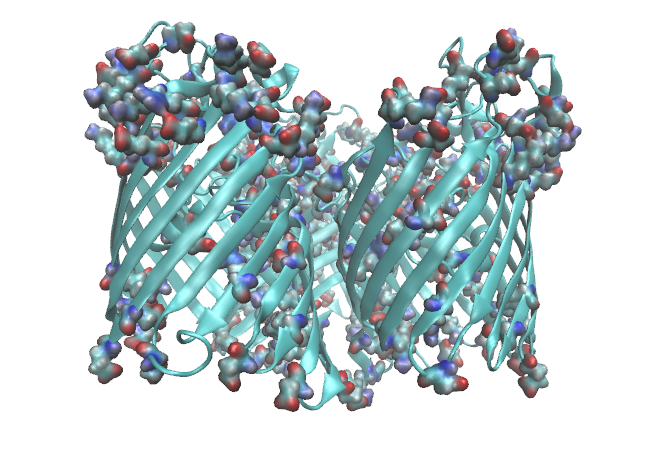
\includegraphics[scale=0.5]{ompf}
\caption{Side-view of structure: three $\beta$-barrels transmembrane channel.\\
Highlighted are charged residues, which dominanate the outer membrane side.}
\label{fig:ompF}
\end{figure}

Every student will find raw data for the following applied voltages: ±100mV,
±200mV, ±1000mV.
For ±100mV: every student will have only 1 trajectory to analyse (the file dcd).
For ±200mV: every student will have 6 trajectories to analyse (the file dcd).
For ±1000mV: every student will have 3 trajectories to analyse (the file dcd).
Every student is supposed to follow the pipeline of analysis
proposed/provided during the tutorial that permits to estimate the relevant
properties of interest of the system. Read carefully the file README before to
start the analysis!
Calculate and discuss ion flux through the channel as well as its conductance,
putting the results in relation with the current literature.
\begin{figure}[H]
	\centering{}
	\captionsetup{justification=centering}
	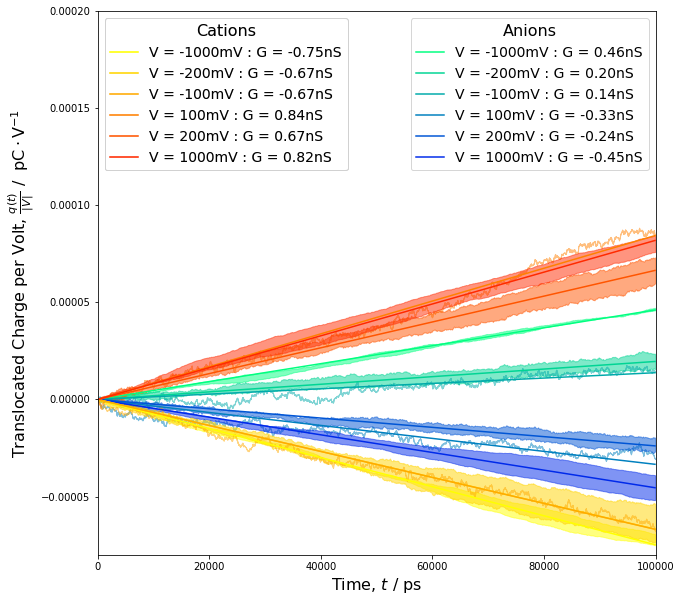
\includegraphics[scale=0.5]{conductance}
\caption{Conductance estimates $G$ for anions and cations across\\ outer membrane
protein F (ompF) under various applied voltages $V$ }
\label{fig:conductance}
\end{figure}

\begin{figure}[H]
	\centering{}
	\captionsetup{justification=centering}
	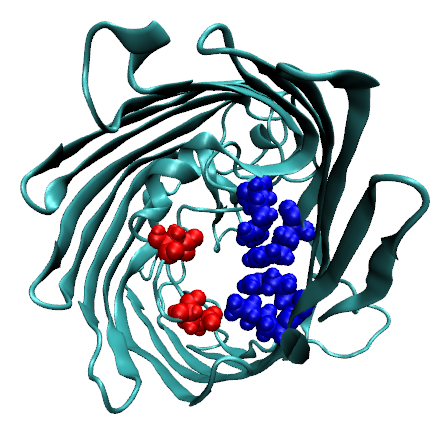
\includegraphics[scale=0.5]{ompf-charges}
\caption{Single ompF $\beta$-barrel from inner membrane side, highlighting
positive  $\mathrm{COOH}$  (red) \\and negative $\mathrm{NH_2}$ (blue) partial charged groups that facilitate cationic selectivity}
\label{fig:ompF-charges}
\end{figure}
The student is supposed to address all the points of the assignment described above,
but has the freedom to focus in discussing details of methodology and selected
approaches either to the “Analysis of Umbrella Sampling Simulations” or to the
“Analysis of the non-equilibrium molecular dynamics simulations with external electric
field”.
\bibliography{mendeley_v2}
\bibliographystyle{ieeetr}
\end{document}
